\documentclass{article}
\usepackage{ctex}
\usepackage{bm}
\usepackage[colorlinks, linkcolor=blue]{hyperref}
\usepackage{geometry}
\geometry{left=3cm, right=3cm, top=3cm, bottom=3cm}
\usepackage{amsmath}
\usepackage{amsthm}
\usepackage[T1]{fontenc}
\usepackage{xcolor}
\usepackage{lmodern}
\usepackage{listings}

\newtheorem{task}{任务}

\lstset{
	numbers=left, 
	numberstyle= \small, 
	keywordstyle= \color{ blue!70},
	commentstyle= \color{red!50!green!50!blue!50}, 
	frame=shadowbox, % 阴影效果
	showstringspaces = false,
	flexiblecolumns,                % 别问为什么,加上这个
	rulesepcolor= \color{ red!20!green!20!blue!20} ,
	escapeinside=``, % 英文分号中可写入中文
	xleftmargin=2em,xrightmargin=2em, aboveskip=1em,
	framexleftmargin=2em
}

\lstdefinestyle{Fortran}{
	language        =   [90]Fortran,
	basicstyle=\small\ttfamily
}

\title{作业一:Fortran 编程练习}
\author{英才1701 赵鹏威 U201710152}

\begin{document}
	\maketitle
	\tableofcontents
	\newpage
	\section{引言}
	Fortran 是最早面世的高级编程语言,名字的来源是 Formula Translator,在科学计算方面有很广泛的运用. 虽然 Fortran 十分古老,但是早期许多优秀的数值计算程序都是基于 Fortran 代码编写的,因此熟悉 Fortran 语言是十分有帮助的. 另外,Fortran 语言具有高效率的优势,这一点与 C/C++ 相似,但是 Fortran 中内置了许多数学函数,使用 Fortran 编写的数值计算程序要相对简洁不少. 本次作业的目的就是熟悉 Fortran 语言的基础语法,包括基本的输入输出、文件读写、数组运算等内容.
	
	\section{基本的输入输出}
	\subsection{任务描述}
	\begin{task}
		编写 Fortran 程序实现以下功能:
		\begin{itemize}
			\item 程序能读取用户输入的矩阵;
			\item 输入矩阵后,程序可以将矩阵保存到一个文本文件中;
			\item 程序能从文本文件中读取矩阵;
			\item 程序能按照固定的格式打印矩阵到屏幕上.
		\end{itemize}
	\end{task}
	一个好的程序要有适当的泛化能力. 考虑到用户输入的矩阵大小不确定,因此编写的程序需要适应各种大小的矩阵. 在输入矩阵时,用户需要先输入矩阵的大小,也就是有多少行和多少列.
	\subsection{程序实现}
	程序需要四个功能:输入矩阵、写入文件、读取文件、打印矩阵. ”输入矩阵“使用一个 function 实现,这个调用这个 function 后,程序会要求用户输入矩阵的大小,然后按行输入矩阵. 这个 function 返回一个二位数组,其保存着用户输入的矩阵. 让用户输入矩阵大小的功能可以用动态数组实现,也可以预先定义一个大小较大的二维数组来实现,这里采用后一种方法,也就是预先定义一个 $100\times100$ 的二位数组,这样用户可以输入比这个大小小的任意矩阵. “写入矩阵”和“读取文件”矩阵分别使用一个 subroutine 实现. 写入、读取和打印矩阵时使用格式输出,程序先获取矩阵的大小,然后按照固定的格式写入、读取和打印矩阵. 由于,输入矩阵的 function 需要返回一个数组,因此将实现上面三个功能的 function 和 subroutine 封装在同一个 module 中. 程序代码见附录 Listing \ref{io.f90}. 整个程序的工作流程图见图 \ref{fig:io}.
	\begin{figure}[h!tb]
		\centering
		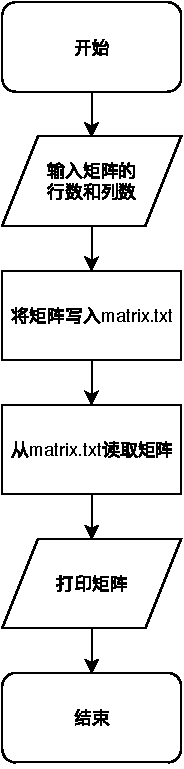
\includegraphics[width=0.2\textwidth]{./utils/io.pdf}
		\caption{ 任务1程序的流程图\label{fig:io}}
	\end{figure}
	\subsection{运行时结果}
	运行附录 Listing \ref{io.f90} 所示代码,运行时结果如图 \ref{fig:rtr_io}. 确保程序确实正确地将矩阵写入了 matrix.txt 文件,打开看到确实正常写入,见图 \ref{fig:matrix}.
	\begin{figure}[h!tb]
		\centering
		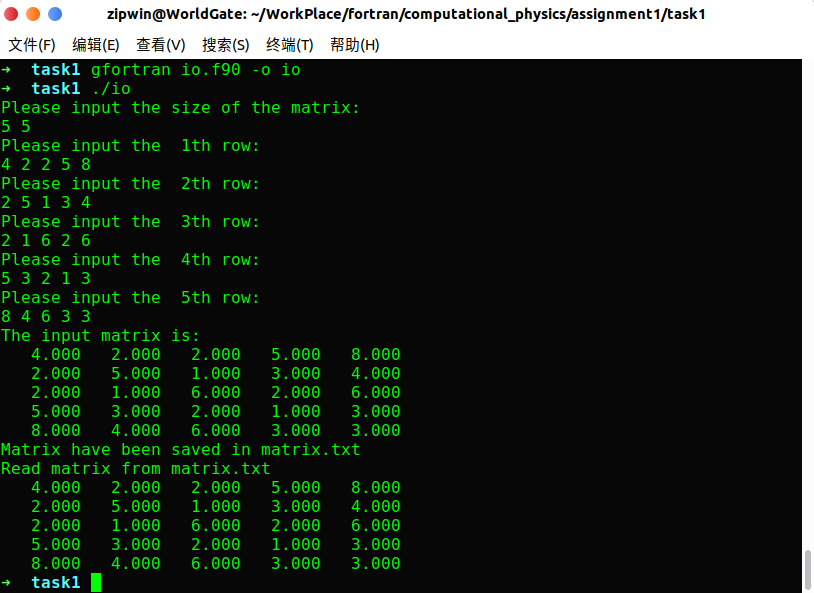
\includegraphics[width=0.8\textwidth]{./utils/rtr_io.png}
		\caption{ 任务1运行时结果\label{fig:rtr_io}}
	\end{figure}
	\begin{figure}[h!tb]
		\centering
		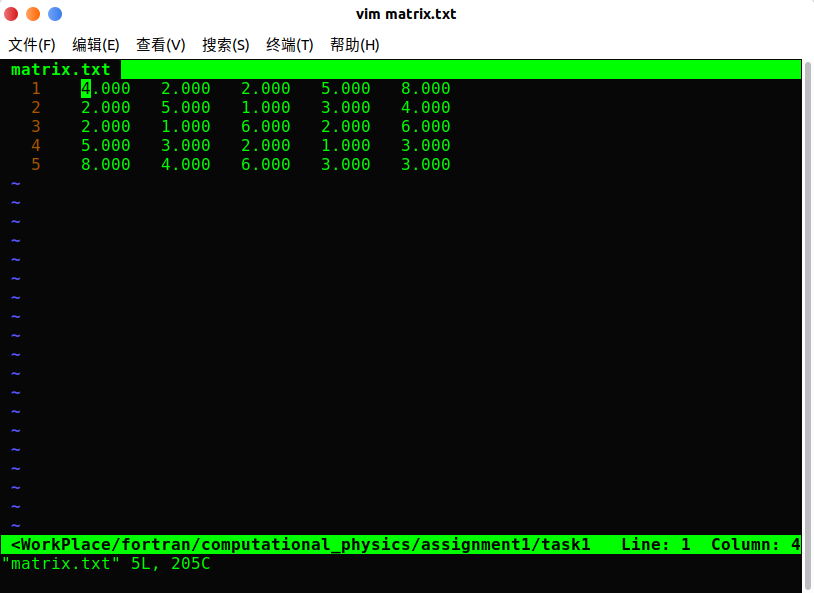
\includegraphics[width=0.8\textwidth]{./utils/matrix.png}
		\caption{ 任务1写入 matrix.txt 的内容\label{fig:matrix}}
	\end{figure}

	\section{矩阵乘法}
	\subsection{任务描述}
	\begin{task}
		给定矩阵$\bm{A}$和列向量$\bm{b}$,使用 subroutine 计算$\bm{Ab}$和$\bm{b}^T\bm{A}\bm{b}$. 其中
		\[
		\bm{A} = 
		\begin{bmatrix}
		4 & 2 & 2 & 5 & 8 \\
		2 & 5 & 1 & 3 & 4 \\
		2 & 1 & 6 & 2 & 6 \\
		5 & 3 & 2 & 1 & 3 \\
		8 & 4 & 6 & 3 & 3
		\end{bmatrix}
		\quad
		\bm{b}=
		\begin{bmatrix}
		2 \\
		4 \\
		5 \\
		2 \\
		1 \\
		\end{bmatrix}
		\]
	\end{task}
	\subsection{程序实现}
	Fortran 自带矩阵乘法函数 matmul(matrix1, matrix2),和转置 transpose(matrix). 列向量可以看做是$n\times1$维的矩阵,因此需要定义两个二维数组来完成这一程序. 由于 subroutine 没有返回值,需要输出的变量都是要在主程序定义好再作为参数传递给 subroutine 的,因此为了便于区分输入参数和输出参数,将输出参数写在输入参数后面. 程序的流程图如图 \ref{fig:matrix_algebra} 所示. 代码见附录 Listing \ref{matrix_algebra.f90}.
	\begin{figure}[h!tb]
		\centering
		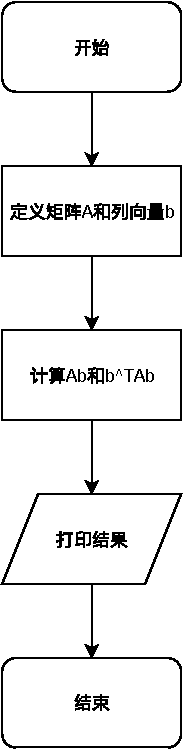
\includegraphics[width=0.2\textwidth]{./utils/matrix_algebra.pdf}
		\caption{ 任务2程序流程图\label{fig:matrix_algebra}}
	\end{figure}
	\subsection{运行时结果}
	为了检验程序计算结果的正确性,手动计算得到解析结果如下
	\[
	\bm{A}\bm{b}=
	\begin{bmatrix}
	44 \\
	39 \\
	48 \\
	37 \\
	71
	\end{bmatrix}
	\quad
	\bm{b}^T\bm{A}\bm{b}=629
	\]
	程序运行时结果如图 \ref{fig:matrix_algebra} 所示. 可见程序计算结果正确. 
	\begin{figure}[h!tb]
		\centering
		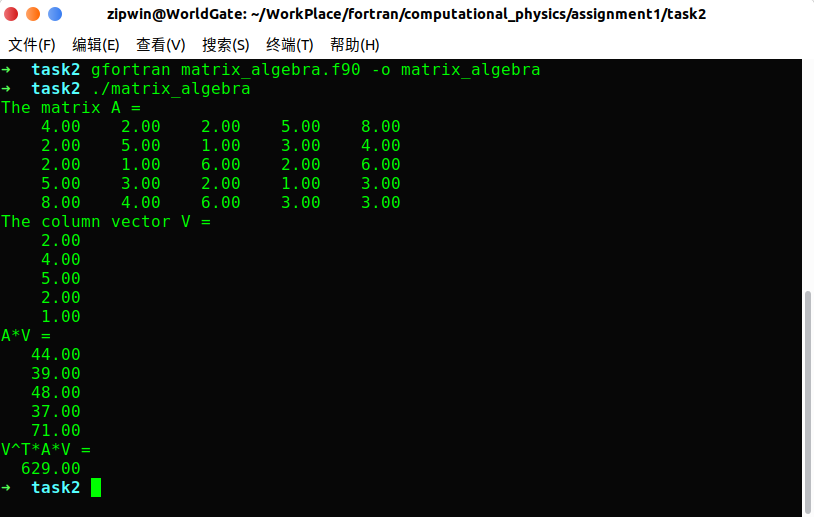
\includegraphics[width=0.8\textwidth]{./utils/rtr_matrix_algebra.png}
		\caption{ 任务2运行时结果\label{fig:rtr_matrix_algebra}}
	\end{figure}
	
	\section{排列数和组合数计算}
	\subsection{任务描述}
	\begin{task}
		给定$n=12, m=8$,编写 subroutine 计算排列数$P_n^m$和组合数$C_n^m$
		\[
		P_n^m=\frac{n!}{(n-m)!}\quad C_n^m=\frac{n!}{m!(n-m)!}
		\]
	\end{task}
	如果直接计算阶乘,会遇到溢出的错误. 4 字节整数最大能储存$2^15-1=32767$, 8 字节整数最大能储存$2^31-1=2.1475e+09$. 而$8!=4032$已经超过了4字节整数的容量,并且$13!=6.2270e+09$也超过了8字节整数的容量. 可见不能直接计算阶乘,而应该在计算之前尽可能约分.
	\subsection{程序实现}
	为了方便与简洁,先写了一个名为 mul2 的函数,这个函数 可以计算$n,m$之间所有整数的积(包括$n,m$). 这个子程序使用递归实现,代码如下(Listing \ref{mul2.f90})
	\lstinputlisting[
	style = Fortran,
	caption     =   {\bf mul2},
	label       =   {mul2.f90}
	]{./utils/mul2.f90}
	这个函数在$n$的值比$m$小时输出$1$.
	
	按照上面所分析的,在计算排列数和组合数之前先约分的方法,可以把排列数的公式改写成
	\[
	P_n^m=\mathrm{mul2}(n, n-m+1)
	\]
	同样组合数也可以改写为
	\[
	C_n^m=
	\begin{cases}
		&\frac{\mathrm{mul2}(n, m+1)}{\mathrm{mul2}(n-m, 1)} \quad m\ge \frac{n}{2} \\
		&\frac{\mathrm{mul2}(n, n-m+1)}{\mathrm{mul2}(m, 1)} \quad m<\frac{n}{2}
	\end{cases}
	\]
	这样就可以尽可能地防止内存溢出. 另外,计算排列数和组合数的子程序在输入不合法时($m<0$或$n<m$)会输出错误信息. 整个程序的流程图如图 \ref{fig:perm_and_comb} 所示,代码见附录 Listing \ref{perm_and_comb.f90}. 
	\begin{figure}[h!tb]
		\centering
		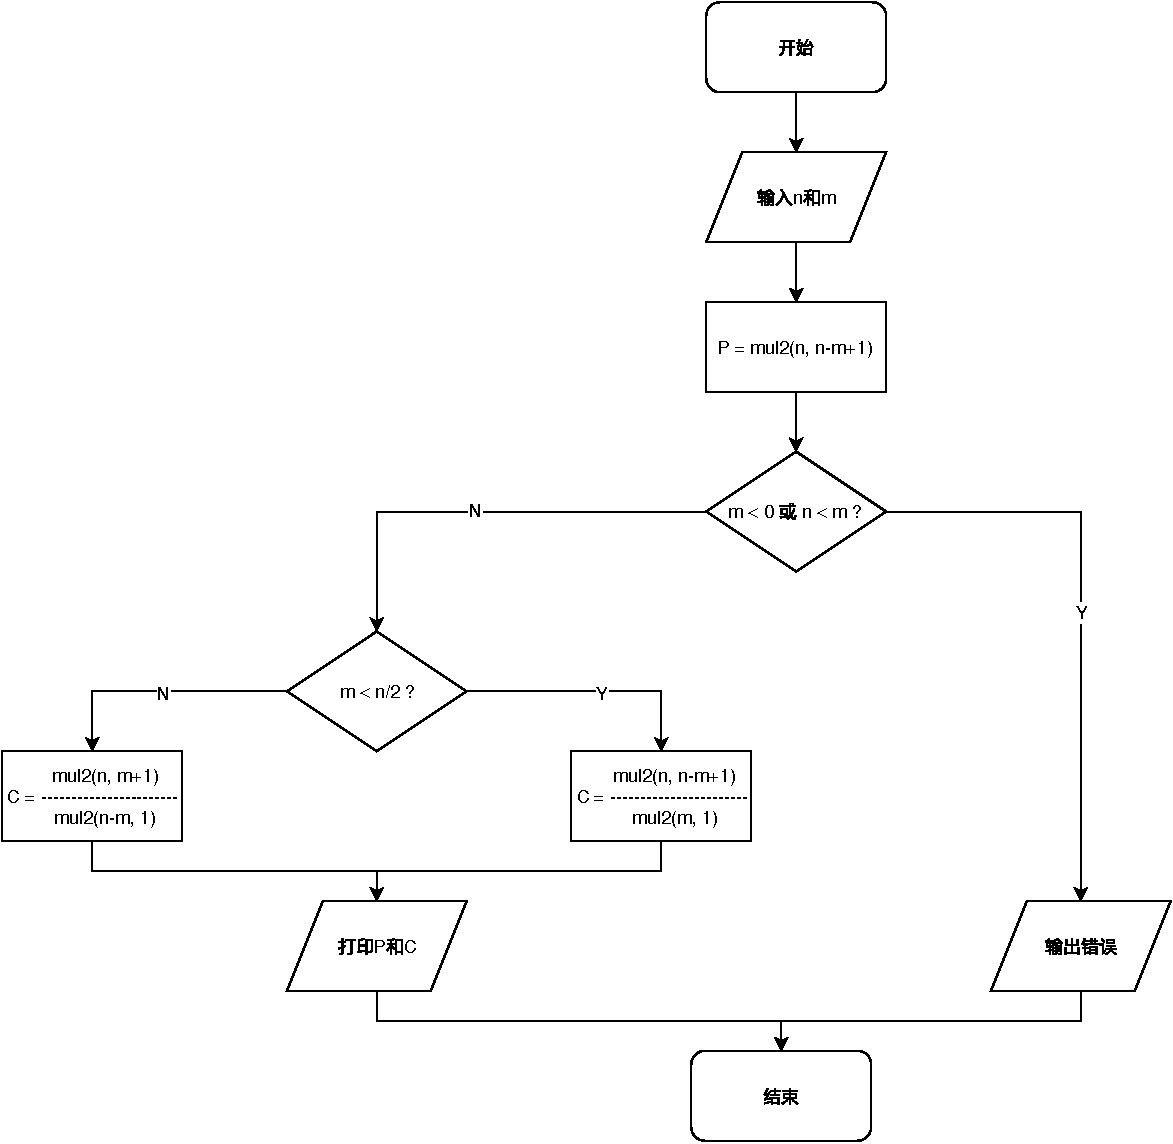
\includegraphics[width=0.7\textwidth]{./utils/perm_and_comb.pdf}
		\caption{ 任务3程序流程图\label{fig:perm_and_comb}}
	\end{figure}
	\subsection{运行时结果}
	输入$n=12,m=8$,程序计算得到的结果如图 \ref{fig:rtr_pc} 所示. 得到的结果是,排列数为$19958400$,组合数为$495$. 利用 Octave 计算的值也分别是$19958400$和$495$,可见程序的计算结果是正确的.
	\begin{figure}[h!tb]
		\centering
		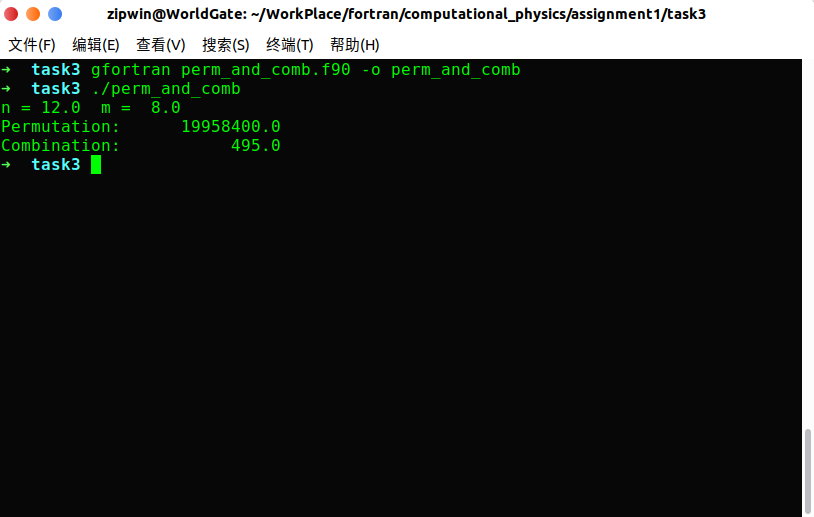
\includegraphics[width=0.8\textwidth]{./utils/rtr_pc.png}
		\caption{ 任务3运行时结果\label{fig:rtr_pc}}
	\end{figure}
	
	\newpage
	\section*{附录}
	这次作业的代码可以在
	\lstinputlisting[
	style = Fortran,
	caption     =   {\bf 任务1 基本输入输出 io.f90},
	label       =   {io.f90}
	]{./utils/io.f90}
	
	\newpage
	\lstinputlisting[
	style = Fortran,
	caption     =   {\bf 任务2 矩阵乘法 matrix\_algebra.f90},
	label       =   {matrix_algebra.f90}
	]{./utils/matrix_algebra.f90}
	
	\newpage
	\lstinputlisting[
	style = Fortran,
	caption     =   {\bf 任务3 排列数和组合数 perm\_and\_comb.f90},
	label       =   {perm_and_comb.f90}
	]{./utils/perm_and_comb.f90}
	
\end{document}